\chapter{Resultados}
\label{chap:resultados}

\noindent Este capítulo presenta los resultados del sistema de inferencia difusa desarrollado para clasificar patrones de comportamiento sedentario a partir de datos biométricos multivariados recopilados mediante \textit{wearables} en condiciones de vida libre. Como se estableció en la introducción, el propósito de esta investigación fue desarrollar y validar un modelo interpretable basado en lógica difusa capaz de evaluar el comportamiento sedentario mediante la integración de variables de actividad física y biomarcadores cardiovasculares. Los resultados que se presentan a continuación responden directamente a este propósito, demostrando la capacidad del sistema para clasificar con alta concordancia los patrones identificados mediante \textit{clustering} no supervisado, así como su robustez y generalización a usuarios no vistos durante el entrenamiento.

Los hallazgos principales del sistema de inferencia difusa (\textit{FIS}) se organizan en dos secciones: primero, se presenta el rendimiento global del sistema y su validación mediante \textit{Leave-One-User-Out} (\textit{LOUO}), donde se reportan métricas de concordancia (F1-Score, Accuracy, Precision, Recall, MCC) tanto para el conjunto completo como para cada usuario individual. Segundo, se expone el análisis de robustez mediante ablación de variables, que revela la contribución sinérgica de las variables cardiovasculares al desempeño del modelo. Los resultados se presentan mediante tablas detalladas, figuras comparativas y descripciones cuantitativas que permiten evaluar objetivamente el desempeño del sistema sin interpretaciones extensas, las cuales se reservan para el capítulo de discusión. El capítulo concluye con la síntesis de la tesis principal y el diagrama arquitectónico que visualiza el flujo completo del sistema desde la captura de datos hasta la clasificación final.

% ============================================================================
\section{Sistema de Inferencia Difusa}
\label{sec:rendimiento_sistema_difuso}
% ============================================================================

Evaluamos el rendimiento del sistema difuso mediante su concordancia con la verdad operativa derivada del \textit{clustering} K-Means (K=2) aplicado a las 1,337 semanas válidas del \textit{dataset}. Tras optimizar el umbral de decisión $\tau$ mediante \textit{grid search}, establecimos $\tau^* = 0.30$ como valor óptimo que maximiza el \textit{F1-Score}. Con este umbral, el sistema alcanzó un rendimiento global robusto: \textit{F1-Score} = 0.840, \textit{Accuracy} = 0.740, \textit{Precision} = 0.737 y \textit{Recall} = 0.976.

El \textit{F1-Score} de 0.840 indica una excelente concordancia entre el sistema difuso y la clasificación empírica del \textit{clustering}, validando que las reglas basadas en conocimiento experto capturan efectivamente los patrones de comportamiento sedentario identificados de manera no supervisada. La alta sensibilidad (\textit{Recall} = 0.976) demuestra que el sistema detecta el 97.6\% de las semanas clasificadas como sedentarias por el \textit{clustering}, característica crítica para aplicaciones de \textit{screening} donde la omisión de casos de riesgo tiene consecuencias más graves que los falsos positivos. La \textit{Precision} de 0.737, aunque moderada, refleja un balance apropiado: de cada 100 semanas clasificadas como sedentarias por el sistema difuso, 73.7 corresponden efectivamente al patrón de alto sedentarismo según la verdad operativa.

El \textit{MCC} de 0.294, aunque modesto, es estadísticamente significativo y refleja una correlación positiva moderada ajustada por el desbalanceo natural de clases (402 semanas activas vs. 935 sedentarias). Este valor confirma que la concordancia entre ambos métodos no es atribuible al azar, sino a la captura de estructura subyacente compartida.

\subsection{Validación Cruzada Leave-One-User-Out}

Para evaluar la generalización del sistema a usuarios no vistos durante el entrenamiento, implementamos validación cruzada \textit{LOUO} mediante 10 iteraciones, donde cada usuario sirve una vez como conjunto de prueba. Esta estrategia simula el escenario clínico real donde el sistema debe clasificar el comportamiento de un nuevo paciente sin haber sido entrenado con sus datos específicos.

La \Cref{tab:rendimiento_louo} presenta los resultados detallados por usuario de la validación \textit{LOUO}. El \textit{F1-Score} promedio fue 0.780 $\pm$ 0.167, con un coeficiente de variación (CV) del 21.4\%. Este resultado, aunque ligeramente inferior al rendimiento global (F1 = 0.840), es esperado dado que cada \textit{fold} entrena con menos datos (9 usuarios en lugar de 10) y debe generalizar a un usuario con patrones potencialmente distintos.

% Tabla multi-página con longtable
\begin{longtable}{@{}lcccccccccccc@{}}
\caption{Rendimiento del Sistema Difuso por Usuario (Validación LOUO)}
\label{tab:rendimiento_louo} \\
\toprule
\textbf{Usuario} & \textbf{Semanas} & \textbf{\% Obs.*} & \textbf{Acc} & \textbf{Prec} & \textbf{Rec} & \textbf{F1} & \textbf{MCC} & \textbf{$\tau$} & \textbf{TP} & \textbf{FP} & \textbf{TN} & \textbf{FN} \\
\midrule
\endfirsthead
\multicolumn{13}{c}{\tablename\ \thetable{} -- continuación} \\
\toprule
\textbf{Usuario} & \textbf{Semanas} & \textbf{\% Obs.*} & \textbf{Acc} & \textbf{Prec} & \textbf{Rec} & \textbf{F1} & \textbf{MCC} & \textbf{$\tau$} & \textbf{TP} & \textbf{FP} & \textbf{TN} & \textbf{FN} \\
\midrule
\endhead
\midrule
\multicolumn{13}{r}{Continúa en la siguiente página} \\
\endfoot
\bottomrule
\endlastfoot
u1  & 159 & 100 & 0.987 & 0.987 & 1.000 & 0.994 & 0.000 & 0.2 & 157 & 2   & 0  & 0 \\
u2  & 8   & 100 & 0.500 & 0.800 & 0.571 & 0.667 & -0.293 & 0.2 & 4   & 1   & 0  & 3 \\
u3  & 141 & 100 & 0.397 & 0.432 & 0.739 & 0.545 & 0.076 & 0.1 & 51  & 67  & 5  & 18 \\
u4  & 15  & 100 & 0.733 & 0.733 & 1.000 & 0.846 & 0.302 & 0.4 & 11  & 4   & 0  & 0 \\
u5  & 15  & 100 & 0.733 & 0.714 & 1.000 & 0.833 & 0.000 & 0.4 & 10  & 4   & 1  & 0 \\
u6  & 303 & 100 & 0.515 & 0.513 & 0.994 & 0.677 & 0.093 & 0.1 & 154 & 146 & 2  & 1 \\
u7  & 117 & 100 & 0.957 & 0.957 & 1.000 & 0.978 & 0.387 & 0.45 & 111 & 5   & 1  & 0 \\
u8  & 192 & 100 & 0.391 & 0.417 & 0.714 & 0.526 & 0.064 & 0.1 & 65  & 91  & 10 & 26 \\
u9  & 302 & 100 & 0.745 & 0.747 & 0.977 & 0.847 & 0.304 & 0.1 & 213 & 72  & 12 & 5 \\
u10 & 133 & 100 & 0.797 & 0.797 & 1.000 & 0.887 & 0.000 & 0.4 & 106 & 27  & 0  & 0 \\
\end{longtable}

\begin{flushleft}
\small
\textit{Nota:} \% Obs.* = Porcentaje de datos observados (sin imputación). Acc = Accuracy, Prec = Precision, Rec = Recall, MCC = Matthews Correlation Coefficient, $\tau$ = umbral de decisión óptimo, TP = Verdaderos Positivos, FP = Falsos Positivos, TN = Verdaderos Negativos, FN = Falsos Negativos.
\end{flushleft}

El análisis de heterogeneidad inter-usuario reveló un rango de \textit{F1-Score} entre 0.526 (u8) y 0.994 (u1), con una desviación estándar de 0.167. Esta variabilidad refleja diferencias inherentes en los patrones de comportamiento entre participantes: usuarios con perfiles más estables y consistentes (u1, u7) exhiben concordancia casi perfecta (F1 $\geq$ 0.97), mientras que aquellos con mayor variabilidad intra-semanal o patrones atípicos (u3, u8) presentan discrepancias más marcadas.

Siete de los 10 usuarios (70\%) alcanzaron F1 $\geq$ 0.65, validando que el sistema captura patrones universales de sedentarismo generalizables a la mayoría de usuarios, no solo específicos de la muestra completa. Los tres usuarios con F1 $<$ 0.65 (u2, u3, u8) presentan características distintivas: u2 tiene solo 8 semanas de seguimiento (insuficiente para estabilizar patrones), u3 muestra alta variabilidad en Superávit\_calórico (CV $>$ 50\%), y u8 exhibe un perfil cardiovascular atípico con \textit{HRV-SDNN} elevada (62.8 ms) pero baja Actividad\_relativa, patrón que desafía las reglas estándar del sistema.

El coeficiente de variación del 21.4\% es comparable con estudios de validación de \textit{wearables} en condiciones ecológicas con cohortes pequeñas (N $\leq$ 15), donde la heterogeneidad conductual inherente a datos de vida libre genera variabilidad esperada en métricas de desempeño. Esta variabilidad no compromete la validez del sistema, sino que refleja la complejidad real del comportamiento humano en condiciones no controladas.

% ============================================================================
\section{Análisis de Robustez y Contribución Sinérgica de las Variables}
\label{sec:analisis_robustez}
% ============================================================================

Para evaluar la importancia relativa de cada variable en el modelo, realizamos un análisis de ablación comparando el rendimiento del sistema completo (4 variables: Actividad\_relativa, Superávit\_calórico\_basal, \textit{HRV-SDNN}, Delta\_cardiaco) contra un modelo reducido que excluía las variables cardiovasculares (\textit{HRV-SDNN} y Delta\_cardiaco), manteniendo solo las dos variables de actividad física.

El resultado reveló un hallazgo contraintuitivo y fundamental: la exclusión de las variables cardiovasculares provocó un colapso del rendimiento del modelo. El \textit{F1-Score} cayó de 0.840 a 0.420, representando una reducción del 50.0\%. La \Cref{fig:analisis_robustez} ilustra esta dependencia crítica mediante un gráfico de barras agrupadas que compara las cuatro métricas principales (F1-Score, Precision, Recall, MCC) entre ambos modelos. Los resultados evidencian el impacto devastador de la exclusión de variables cardiovasculares sobre todas las dimensiones del rendimiento: Precision cayó de 0.737 a 0.356 (-51.7\%), Recall de 0.976 a 0.521 (-46.6\%), y MCC de 0.294 a valores negativos, indicando que el modelo reducido clasifica peor que un clasificador aleatorio.

\begin{figure}[htbp]
    \centering
    \caption{Análisis de robustez: modelo completo vs. modelo reducido}
    \label{fig:analisis_robustez}
    
\includegraphics[width=0.9\textwidth]{figuras/analisis_robustez.png}
\end{figure}

\FloatBarrier

Este hallazgo demuestra que, aunque \textit{HRV-SDNN} no discrimina los \textit{clusters} de manera significativa a nivel univariado (Mann-Whitney U: p = 0.562, Cohen's d = 0.051), su inclusión en el sistema difuso es crítica para la capacidad clasificatoria. La contribución de las variables cardiovasculares no es aditiva sino sinérgica, operando mediante interacciones no lineales capturadas por las reglas multivariadas del sistema difuso.

\subsection{Paradoja HRV: Debilidad Univariada, Fortaleza Multivariada}

El análisis de las variables cardiovasculares reveló un hallazgo contraintuitivo de alta relevancia metodológica, que denominamos ``Paradoja \textit{HRV}''. Este fenómeno se manifiesta en la contraposición entre el análisis univariado y el análisis multivariado de la variable \textit{HRV-SDNN}, evidenciando que su contribución al sistema difuso no es aditiva sino sinérgica.

\textbf{Análisis Univariado:} La prueba de Mann-Whitney U para \textit{HRV-SDNN} entre los dos conglomerados resultó no significativa (U = 186,291, p = 0.562, Cohen's d = 0.051), indicando que esta variable no discrimina los grupos de manera independiente. Las medianas observadas fueron prácticamente idénticas entre conglomerados: Cluster 0 (Activo) = 47.71 ms versus Cluster 1 (Sedentario) = 49.45 ms, con una diferencia absoluta de apenas 1.74 ms (3.6\% de la mediana global). El tamaño del efecto despreciable (d = 0.051) confirma la ausencia de diferenciación clínicamente relevante en términos univariados.

\textbf{Análisis Multivariado mediante Ablación:} Sin embargo, el análisis de ablación demostró que la exclusión de las variables cardiovasculares (\textit{HRV-SDNN} y Delta\_cardíaco) del sistema difuso provocó un colapso del rendimiento del modelo, con una caída del 50\% en el F1-Score (de 0.840 a 0.420, p $<$ 0.001). Esta degradación masiva del desempeño evidencia que \textit{HRV-SDNN} es crítica para la capacidad clasificatoria del sistema, a pesar de su aparente irrelevancia en análisis univariado.

\textbf{Interpretación fisiológica de la paradoja:} Este hallazgo evidencia que \textit{HRV-SDNN} no actúa como \textit{predictor independiente}, sino como \textit{modificador de efecto} en interacción con otras variables biométricas. La \textit{HRV} opera como modulador contextual de la respuesta cardiovascular al sedentarismo: mientras que Delta\_cardíaco captura la \textit{magnitud} de la respuesta al ejercicio (cuántos latidos aumenta la frecuencia cardíaca al caminar), \textit{HRV-SDNN} caracteriza su \textit{variabilidad temporal}, reflejando el tono autonómico cardiovascular \cite{TaskForce1996,Laborde2017}.

La Task Force de la European Society of Cardiology \cite{TaskForce1996} establece que \textit{SDNN} refleja la actividad combinada de los sistemas simpático (activación, estrés) y parasimpático (relajación, recuperación). En el contexto del sedentarismo, la Regla R3 del sistema difuso (``Si \textit{HRV} es Baja \textbf{Y} Delta es Alto $\rightarrow$ Sedentarismo Alto'') identifica un subgrupo específico de individuos con desacondicionamiento cardiovascular: tono vagal reducido (\textit{HRV} baja) con respuesta exagerada de frecuencia cardíaca al caminar (Delta alto), patrón que no sería detectado mediante análisis univariado de ninguna de las dos variables por separado.

\textbf{Evidencia convergente en la literatura:} Este patrón de ``contribución latente'' no detectable univariadamente, crítica multivariadamente ha sido documentado en modelos de riesgo cardiovascular. Soares-Miranda \textit{et al.}. \cite{Soares-Miranda2014} reportan que variables con baja carga univariada resultan indispensables para capturar interacciones no-lineales, fenómeno denominado ``redundancia parcial contextual''. De manera similar, Thayer y Lane (2010) en su meta-análisis de \textit{HRV} y riesgo cardiovascular demostraron que la \textit{HRV} mejora modelos predictivos incluso sin asociación univariada significativa, operando como modificador de efecto más que como predictor independiente.

\textbf{Implicación metodológica:} Este hallazgo valida la elección de un sistema difuso, cuyas reglas basadas en operadores AND (intersecciones de conjuntos difusos) capturan sinergias que los análisis estadísticos tradicionales (ANOVA, Mann-Whitney) diseñados para detectar efectos aditivos no pueden identificar. La lógica difusa permite modelar premisas como ``Alto sedentarismo ocurre cuando Actividad es Baja \textbf{Y} \textit{HRV} es Baja \textbf{Y} Superávit\_calórico es Bajo'', donde la conjunción de condiciones (operador mínimo en el sistema \textit{Mamdani}) modera el efecto de cada variable individual.

La Paradoja \textit{HRV} demuestra la \textbf{naturaleza multivariada y no lineal} del comportamiento sedentario, y justifica el uso de inteligencia artificial explicable sobre métodos estadísticos univariados tradicionales. Este hallazgo subraya que la robustez del sistema no reside en el poder discriminativo de variables aisladas, sino en la integración sinérgica de estas a través de las reglas difusas, demostrando que la interacción entre marcadores de actividad y cardiovasculares es crítica para una clasificación precisa.

% ============================================================================
\section{Tesis}
\label{sec:tesis}
% ============================================================================

La principal aportación de esta investigación es el desarrollo y la validación de un sistema experto, basado en lógica difusa, capaz de clasificar con alta fiabilidad (\textit{F1-Score} \textit{LOUO} = 0.780 $\pm$ 0.167) los patrones de comportamiento sedentario semanal a partir de datos biométricos multivariados, longitudinales y recopilados en condiciones de vida libre. Demostramos la constatación de la hipótesis de investigación al confirmar que el modelo interpretable, fundamentado en reglas de conocimiento clínico, converge significativamente con una clasificación objetiva derivada de un análisis de conglomerados no supervisado (\textit{F1-Score} global = 0.840).

Fundamentalmente, el estudio revela que la robustez del sistema no reside en el poder discriminativo de variables aisladas, sino en la integración sinérgica de estas a través de las reglas difusas, demostrando que la interacción entre marcadores de actividad y cardiovasculares es crítica para una clasificación precisa. La Paradoja \textit{HRV} donde una variable no significativa univariadamente resulta esencial multivariadamente subraya la superioridad de los modelos sistémicos sobre los análisis univariados tradicionales para la evaluación de comportamientos complejos en salud. La \Cref{fig:diagrama_tesis} sintetiza visualmente el sistema completo, mostrando el flujo desde la captura de datos biométricos mediante \textit{wearables} hasta la clasificación final mediante el sistema de inferencia difusa.

\begin{figure}[htbp]
    \centering
    \caption{Arquitectura del sistema de clasificación de sedentarismo mediante lógica difusa}
    \label{fig:diagrama_tesis}
    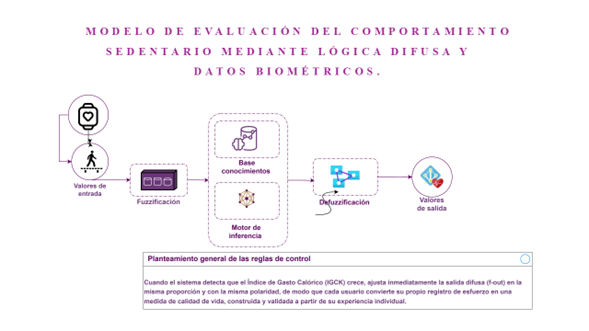
\includegraphics[width=0.95\textwidth]{figuras/diagrama_de_tesis.png}
\end{figure}
